% Created by tikzDevice version 0.12.6 on 2025-10-20 18:47:46
% !TEX encoding = UTF-8 Unicode
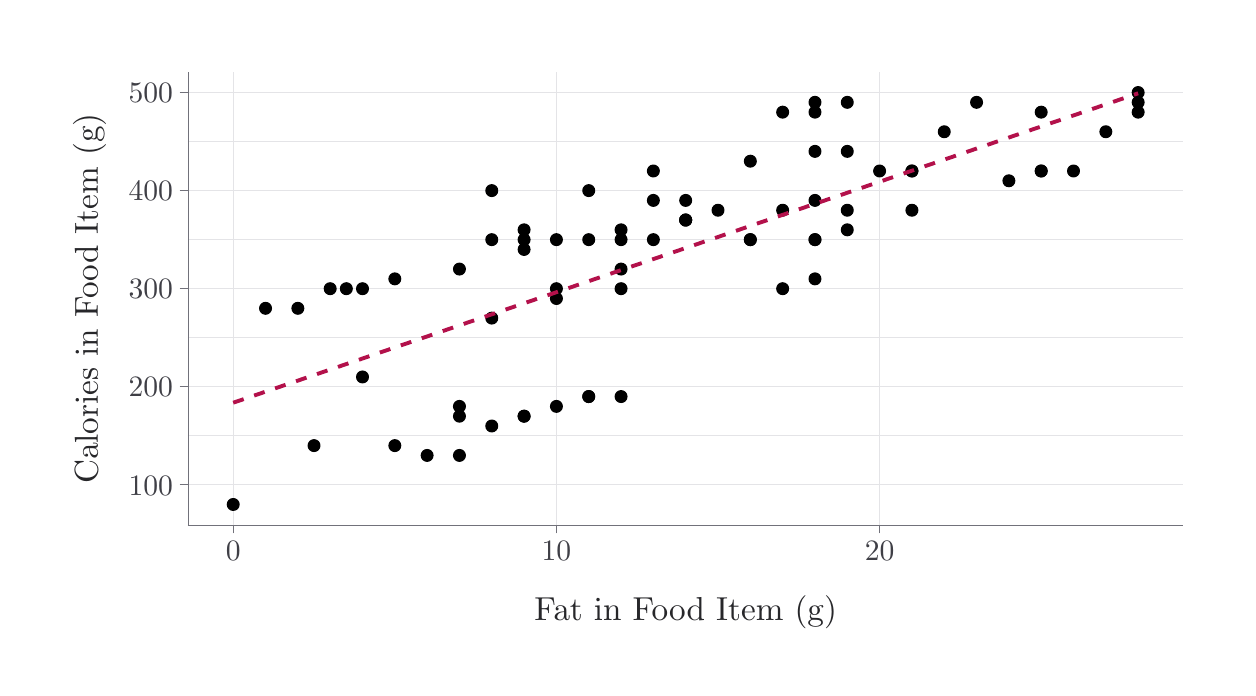
\begin{tikzpicture}[x=1pt,y=1pt]
\definecolor{fillColor}{RGB}{255,255,255}
\path[use as bounding box,fill=fillColor] (0,0) rectangle (433.62,231.26);
\begin{scope}
\path[clip] (  0.00,  0.00) rectangle (433.62,231.26);
\definecolor{drawColor}{RGB}{255,255,255}

\path[draw=drawColor,line width= 0.6pt,line join=round,line cap=round,fill=fillColor] (  0.00,  0.00) rectangle (433.62,231.26);
\end{scope}
\begin{scope}
\path[clip] ( 57.92, 51.53) rectangle (417.62,215.26);
\definecolor{drawColor}{RGB}{255,255,255}
\definecolor{fillColor}{RGB}{255,255,255}

\path[draw=drawColor,line width= 0.6pt,line join=round,line cap=round,fill=fillColor] ( 57.92, 51.53) rectangle (417.62,215.26);
\definecolor{drawColor}{RGB}{228,228,231}

\path[draw=drawColor,line width= 0.4pt,line join=round] ( 57.92, 83.78) --
	(417.62, 83.78);

\path[draw=drawColor,line width= 0.4pt,line join=round] ( 57.92,119.22) --
	(417.62,119.22);

\path[draw=drawColor,line width= 0.4pt,line join=round] ( 57.92,154.66) --
	(417.62,154.66);

\path[draw=drawColor,line width= 0.4pt,line join=round] ( 57.92,190.10) --
	(417.62,190.10);

\path[draw=drawColor,line width= 0.4pt,line join=round] ( 57.92, 66.06) --
	(417.62, 66.06);

\path[draw=drawColor,line width= 0.4pt,line join=round] ( 57.92,101.50) --
	(417.62,101.50);

\path[draw=drawColor,line width= 0.4pt,line join=round] ( 57.92,136.94) --
	(417.62,136.94);

\path[draw=drawColor,line width= 0.4pt,line join=round] ( 57.92,172.38) --
	(417.62,172.38);

\path[draw=drawColor,line width= 0.4pt,line join=round] ( 57.92,207.82) --
	(417.62,207.82);

\path[draw=drawColor,line width= 0.4pt,line join=round] ( 74.27, 51.53) --
	( 74.27,215.26);

\path[draw=drawColor,line width= 0.4pt,line join=round] (191.06, 51.53) --
	(191.06,215.26);

\path[draw=drawColor,line width= 0.4pt,line join=round] (307.84, 51.53) --
	(307.84,215.26);
\definecolor{drawColor}{RGB}{0,0,0}
\definecolor{fillColor}{RGB}{0,0,0}

\path[draw=drawColor,line width= 0.4pt,line join=round,line cap=round,fill=fillColor] (167.70,154.66) circle (  2.14);

\path[draw=drawColor,line width= 0.4pt,line join=round,line cap=round,fill=fillColor] (179.38,154.66) circle (  2.14);

\path[draw=drawColor,line width= 0.4pt,line join=round,line cap=round,fill=fillColor] (307.84,179.47) circle (  2.14);

\path[draw=drawColor,line width= 0.4pt,line join=round,line cap=round,fill=fillColor] (296.16,204.28) circle (  2.14);

\path[draw=drawColor,line width= 0.4pt,line join=round,line cap=round,fill=fillColor] (144.34, 76.69) circle (  2.14);

\path[draw=drawColor,line width= 0.4pt,line join=round,line cap=round,fill=fillColor] (237.77,161.75) circle (  2.14);

\path[draw=drawColor,line width= 0.4pt,line join=round,line cap=round,fill=fillColor] (331.20,193.65) circle (  2.14);

\path[draw=drawColor,line width= 0.4pt,line join=round,line cap=round,fill=fillColor] (237.77,161.75) circle (  2.14);

\path[draw=drawColor,line width= 0.4pt,line join=round,line cap=round,fill=fillColor] (284.49,140.49) circle (  2.14);

\path[draw=drawColor,line width= 0.4pt,line join=round,line cap=round,fill=fillColor] (366.23,179.47) circle (  2.14);

\path[draw=drawColor,line width= 0.4pt,line join=round,line cap=round,fill=fillColor] (272.81,165.29) circle (  2.14);

\path[draw=drawColor,line width= 0.4pt,line join=round,line cap=round,fill=fillColor] (214.42,144.03) circle (  2.14);

\path[draw=drawColor,line width= 0.4pt,line join=round,line cap=round,fill=fillColor] (272.81,136.94) circle (  2.14);

\path[draw=drawColor,line width= 0.4pt,line join=round,line cap=round,fill=fillColor] (319.52,179.47) circle (  2.14);

\path[draw=drawColor,line width= 0.4pt,line join=round,line cap=round,fill=fillColor] (132.67,140.49) circle (  2.14);

\path[draw=drawColor,line width= 0.4pt,line join=round,line cap=round,fill=fillColor] (284.49,200.73) circle (  2.14);

\path[draw=drawColor,line width= 0.4pt,line join=round,line cap=round,fill=fillColor] (284.49,204.28) circle (  2.14);

\path[draw=drawColor,line width= 0.4pt,line join=round,line cap=round,fill=fillColor] (354.56,175.93) circle (  2.14);

\path[draw=drawColor,line width= 0.4pt,line join=round,line cap=round,fill=fillColor] (156.02, 76.69) circle (  2.14);

\path[draw=drawColor,line width= 0.4pt,line join=round,line cap=round,fill=fillColor] ( 97.63,129.85) circle (  2.14);

\path[draw=drawColor,line width= 0.4pt,line join=round,line cap=round,fill=fillColor] (214.42,158.21) circle (  2.14);

\path[draw=drawColor,line width= 0.4pt,line join=round,line cap=round,fill=fillColor] (342.88,204.28) circle (  2.14);

\path[draw=drawColor,line width= 0.4pt,line join=round,line cap=round,fill=fillColor] (366.23,179.47) circle (  2.14);

\path[draw=drawColor,line width= 0.4pt,line join=round,line cap=round,fill=fillColor] (284.49,186.56) circle (  2.14);

\path[draw=drawColor,line width= 0.4pt,line join=round,line cap=round,fill=fillColor] (226.09,154.66) circle (  2.14);

\path[draw=drawColor,line width= 0.4pt,line join=round,line cap=round,fill=fillColor] (120.99,105.05) circle (  2.14);

\path[draw=drawColor,line width= 0.4pt,line join=round,line cap=round,fill=fillColor] (261.13,154.66) circle (  2.14);

\path[draw=drawColor,line width= 0.4pt,line join=round,line cap=round,fill=fillColor] (109.31,136.94) circle (  2.14);

\path[draw=drawColor,line width= 0.4pt,line join=round,line cap=round,fill=fillColor] (319.52,179.47) circle (  2.14);

\path[draw=drawColor,line width= 0.4pt,line join=round,line cap=round,fill=fillColor] (237.77,161.75) circle (  2.14);

\path[draw=drawColor,line width= 0.4pt,line join=round,line cap=round,fill=fillColor] (132.67, 80.24) circle (  2.14);

\path[draw=drawColor,line width= 0.4pt,line join=round,line cap=round,fill=fillColor] ( 85.95,129.85) circle (  2.14);

\path[draw=drawColor,line width= 0.4pt,line join=round,line cap=round,fill=fillColor] (237.77,168.84) circle (  2.14);

\path[draw=drawColor,line width= 0.4pt,line join=round,line cap=round,fill=fillColor] (272.81,200.73) circle (  2.14);

\path[draw=drawColor,line width= 0.4pt,line join=round,line cap=round,fill=fillColor] (366.23,200.73) circle (  2.14);

\path[draw=drawColor,line width= 0.4pt,line join=round,line cap=round,fill=fillColor] (261.13,183.01) circle (  2.14);

\path[draw=drawColor,line width= 0.4pt,line join=round,line cap=round,fill=fillColor] (167.70,172.38) circle (  2.14);

\path[draw=drawColor,line width= 0.4pt,line join=round,line cap=round,fill=fillColor] (179.38,151.12) circle (  2.14);

\path[draw=drawColor,line width= 0.4pt,line join=round,line cap=round,fill=fillColor] (191.06,154.66) circle (  2.14);

\path[draw=drawColor,line width= 0.4pt,line join=round,line cap=round,fill=fillColor] (296.16,186.56) circle (  2.14);

\path[draw=drawColor,line width= 0.4pt,line join=round,line cap=round,fill=fillColor] (401.27,204.28) circle (  2.14);

\path[draw=drawColor,line width= 0.4pt,line join=round,line cap=round,fill=fillColor] (401.27,200.73) circle (  2.14);

\path[draw=drawColor,line width= 0.4pt,line join=round,line cap=round,fill=fillColor] (167.70,126.31) circle (  2.14);

\path[draw=drawColor,line width= 0.4pt,line join=round,line cap=round,fill=fillColor] (296.16,158.21) circle (  2.14);

\path[draw=drawColor,line width= 0.4pt,line join=round,line cap=round,fill=fillColor] (249.45,165.29) circle (  2.14);

\path[draw=drawColor,line width= 0.4pt,line join=round,line cap=round,fill=fillColor] (296.16,165.29) circle (  2.14);

\path[draw=drawColor,line width= 0.4pt,line join=round,line cap=round,fill=fillColor] (377.91,179.47) circle (  2.14);

\path[draw=drawColor,line width= 0.4pt,line join=round,line cap=round,fill=fillColor] (202.74,154.66) circle (  2.14);

\path[draw=drawColor,line width= 0.4pt,line join=round,line cap=round,fill=fillColor] (319.52,165.29) circle (  2.14);

\path[draw=drawColor,line width= 0.4pt,line join=round,line cap=round,fill=fillColor] (156.02, 94.41) circle (  2.14);

\path[draw=drawColor,line width= 0.4pt,line join=round,line cap=round,fill=fillColor] (179.38, 90.87) circle (  2.14);

\path[draw=drawColor,line width= 0.4pt,line join=round,line cap=round,fill=fillColor] (214.42, 97.96) circle (  2.14);

\path[draw=drawColor,line width= 0.4pt,line join=round,line cap=round,fill=fillColor] (156.02, 90.87) circle (  2.14);

\path[draw=drawColor,line width= 0.4pt,line join=round,line cap=round,fill=fillColor] (202.74, 97.96) circle (  2.14);

\path[draw=drawColor,line width= 0.4pt,line join=round,line cap=round,fill=fillColor] (191.06, 94.41) circle (  2.14);

\path[draw=drawColor,line width= 0.4pt,line join=round,line cap=round,fill=fillColor] (167.70, 87.33) circle (  2.14);

\path[draw=drawColor,line width= 0.4pt,line join=round,line cap=round,fill=fillColor] (202.74, 97.96) circle (  2.14);

\path[draw=drawColor,line width= 0.4pt,line join=round,line cap=round,fill=fillColor] (179.38, 90.87) circle (  2.14);

\path[draw=drawColor,line width= 0.4pt,line join=round,line cap=round,fill=fillColor] (284.49,154.66) circle (  2.14);

\path[draw=drawColor,line width= 0.4pt,line join=round,line cap=round,fill=fillColor] (191.06,136.94) circle (  2.14);

\path[draw=drawColor,line width= 0.4pt,line join=round,line cap=round,fill=fillColor] (261.13,154.66) circle (  2.14);

\path[draw=drawColor,line width= 0.4pt,line join=round,line cap=round,fill=fillColor] (401.27,207.82) circle (  2.14);

\path[draw=drawColor,line width= 0.4pt,line join=round,line cap=round,fill=fillColor] (191.06,133.40) circle (  2.14);

\path[draw=drawColor,line width= 0.4pt,line join=round,line cap=round,fill=fillColor] (103.47, 80.24) circle (  2.14);

\path[draw=drawColor,line width= 0.4pt,line join=round,line cap=round,fill=fillColor] (156.02,144.03) circle (  2.14);

\path[draw=drawColor,line width= 0.4pt,line join=round,line cap=round,fill=fillColor] (284.49,154.66) circle (  2.14);

\path[draw=drawColor,line width= 0.4pt,line join=round,line cap=round,fill=fillColor] ( 74.27, 58.97) circle (  2.14);

\path[draw=drawColor,line width= 0.4pt,line join=round,line cap=round,fill=fillColor] (202.74,172.38) circle (  2.14);

\path[draw=drawColor,line width= 0.4pt,line join=round,line cap=round,fill=fillColor] (389.59,193.65) circle (  2.14);

\path[draw=drawColor,line width= 0.4pt,line join=round,line cap=round,fill=fillColor] (179.38,158.21) circle (  2.14);

\path[draw=drawColor,line width= 0.4pt,line join=round,line cap=round,fill=fillColor] (284.49,168.84) circle (  2.14);

\path[draw=drawColor,line width= 0.4pt,line join=round,line cap=round,fill=fillColor] (214.42,154.66) circle (  2.14);

\path[draw=drawColor,line width= 0.4pt,line join=round,line cap=round,fill=fillColor] (226.09,179.47) circle (  2.14);

\path[draw=drawColor,line width= 0.4pt,line join=round,line cap=round,fill=fillColor] (226.09,168.84) circle (  2.14);

\path[draw=drawColor,line width= 0.4pt,line join=round,line cap=round,fill=fillColor] (214.42,136.94) circle (  2.14);

\path[draw=drawColor,line width= 0.4pt,line join=round,line cap=round,fill=fillColor] (120.99,136.94) circle (  2.14);

\path[draw=drawColor,line width= 0.4pt,line join=round,line cap=round,fill=fillColor] (115.15,136.94) circle (  2.14);
\definecolor{drawColor}{RGB}{179,17,75}

\path[draw=drawColor,line width= 1.4pt,dash pattern=on 4pt off 4pt ,line join=round] ( 74.27, 95.74) --
	( 78.41, 97.15) --
	( 82.55, 98.57) --
	( 86.69, 99.98) --
	( 90.83,101.40) --
	( 94.97,102.81) --
	( 99.11,104.23) --
	(103.25,105.64) --
	(107.39,107.06) --
	(111.53,108.47) --
	(115.67,109.89) --
	(119.81,111.30) --
	(123.94,112.72) --
	(128.08,114.13) --
	(132.22,115.55) --
	(136.36,116.96) --
	(140.50,118.38) --
	(144.64,119.79) --
	(148.78,121.21) --
	(152.92,122.63) --
	(157.06,124.04) --
	(161.20,125.46) --
	(165.34,126.87) --
	(169.48,128.29) --
	(173.61,129.70) --
	(177.75,131.12) --
	(181.89,132.53) --
	(186.03,133.95) --
	(190.17,135.36) --
	(194.31,136.78) --
	(198.45,138.19) --
	(202.59,139.61) --
	(206.73,141.02) --
	(210.87,142.44) --
	(215.01,143.85) --
	(219.15,145.27) --
	(223.28,146.68) --
	(227.42,148.10) --
	(231.56,149.51) --
	(235.70,150.93) --
	(239.84,152.34) --
	(243.98,153.76) --
	(248.12,155.17) --
	(252.26,156.59) --
	(256.40,158.00) --
	(260.54,159.42) --
	(264.68,160.84) --
	(268.82,162.25) --
	(272.96,163.67) --
	(277.09,165.08) --
	(281.23,166.50) --
	(285.37,167.91) --
	(289.51,169.33) --
	(293.65,170.74) --
	(297.79,172.16) --
	(301.93,173.57) --
	(306.07,174.99) --
	(310.21,176.40) --
	(314.35,177.82) --
	(318.49,179.23) --
	(322.63,180.65) --
	(326.76,182.06) --
	(330.90,183.48) --
	(335.04,184.89) --
	(339.18,186.31) --
	(343.32,187.72) --
	(347.46,189.14) --
	(351.60,190.55) --
	(355.74,191.97) --
	(359.88,193.38) --
	(364.02,194.80) --
	(368.16,196.22) --
	(372.30,197.63) --
	(376.44,199.05) --
	(380.57,200.46) --
	(384.71,201.88) --
	(388.85,203.29) --
	(392.99,204.71) --
	(397.13,206.12) --
	(401.27,207.54);
\end{scope}
\begin{scope}
\path[clip] (  0.00,  0.00) rectangle (433.62,231.26);
\definecolor{drawColor}{RGB}{113,113,122}

\path[draw=drawColor,line width= 0.3pt,line join=round] ( 57.92, 51.53) --
	( 57.92,215.26);
\end{scope}
\begin{scope}
\path[clip] (  0.00,  0.00) rectangle (433.62,231.26);
\definecolor{drawColor}{RGB}{63,63,70}

\node[text=drawColor,anchor=base east,inner sep=0pt, outer sep=0pt, scale=  1.07] at ( 52.52, 62.39) {100};

\node[text=drawColor,anchor=base east,inner sep=0pt, outer sep=0pt, scale=  1.07] at ( 52.52, 97.83) {200};

\node[text=drawColor,anchor=base east,inner sep=0pt, outer sep=0pt, scale=  1.07] at ( 52.52,133.27) {300};

\node[text=drawColor,anchor=base east,inner sep=0pt, outer sep=0pt, scale=  1.07] at ( 52.52,168.71) {400};

\node[text=drawColor,anchor=base east,inner sep=0pt, outer sep=0pt, scale=  1.07] at ( 52.52,204.15) {500};
\end{scope}
\begin{scope}
\path[clip] (  0.00,  0.00) rectangle (433.62,231.26);
\definecolor{drawColor}{RGB}{113,113,122}

\path[draw=drawColor,line width= 0.3pt,line join=round] ( 54.92, 66.06) --
	( 57.92, 66.06);

\path[draw=drawColor,line width= 0.3pt,line join=round] ( 54.92,101.50) --
	( 57.92,101.50);

\path[draw=drawColor,line width= 0.3pt,line join=round] ( 54.92,136.94) --
	( 57.92,136.94);

\path[draw=drawColor,line width= 0.3pt,line join=round] ( 54.92,172.38) --
	( 57.92,172.38);

\path[draw=drawColor,line width= 0.3pt,line join=round] ( 54.92,207.82) --
	( 57.92,207.82);
\end{scope}
\begin{scope}
\path[clip] (  0.00,  0.00) rectangle (433.62,231.26);
\definecolor{drawColor}{RGB}{113,113,122}

\path[draw=drawColor,line width= 0.3pt,line join=round] ( 57.92, 51.53) --
	(417.62, 51.53);
\end{scope}
\begin{scope}
\path[clip] (  0.00,  0.00) rectangle (433.62,231.26);
\definecolor{drawColor}{RGB}{113,113,122}

\path[draw=drawColor,line width= 0.3pt,line join=round] ( 74.27, 48.53) --
	( 74.27, 51.53);

\path[draw=drawColor,line width= 0.3pt,line join=round] (191.06, 48.53) --
	(191.06, 51.53);

\path[draw=drawColor,line width= 0.3pt,line join=round] (307.84, 48.53) --
	(307.84, 51.53);
\end{scope}
\begin{scope}
\path[clip] (  0.00,  0.00) rectangle (433.62,231.26);
\definecolor{drawColor}{RGB}{63,63,70}

\node[text=drawColor,anchor=base,inner sep=0pt, outer sep=0pt, scale=  1.07] at ( 74.27, 38.78) {0};

\node[text=drawColor,anchor=base,inner sep=0pt, outer sep=0pt, scale=  1.07] at (191.06, 38.78) {10};

\node[text=drawColor,anchor=base,inner sep=0pt, outer sep=0pt, scale=  1.07] at (307.84, 38.78) {20};
\end{scope}
\begin{scope}
\path[clip] (  0.00,  0.00) rectangle (433.62,231.26);
\definecolor{drawColor}{RGB}{39,39,42}

\node[text=drawColor,anchor=base,inner sep=0pt, outer sep=0pt, scale=  1.20] at (237.77, 17.13) {Fat in Food Item (g)};
\end{scope}
\begin{scope}
\path[clip] (  0.00,  0.00) rectangle (433.62,231.26);
\definecolor{drawColor}{RGB}{39,39,42}

\node[text=drawColor,rotate= 90.00,anchor=base,inner sep=0pt, outer sep=0pt, scale=  1.20] at ( 25.39,133.40) {Calories in Food Item (g)};
\end{scope}
\end{tikzpicture}
